\subsection{Risks and Challenges}

\subsubsection{Solar Power}

Solar panel adoption in the United States is increasing year-upon-year, which (depending on solar isolation) can cause `back-feed' events occurring like in Figure \ref{fig:solar}.
An Energy Storage System would benefit in this case as the energy back-fed can be stored for later usage, in a similar way to how the wind turbines perform.
The challenge associated with this model is that since wind and load effects were considered, the MPC's disturbance prediction would have to incorporate the power supplied by solar panels as well, to ensure accurate control.
As visible on the Figure \ref{fig:solar}, this is changing significantly every year, so more research would be required for this case.
Another implication is that fewer wind turbines would be required, and the plant may end up generating excess Hydrogen and Ammonia.
\begin{figure}[htb]
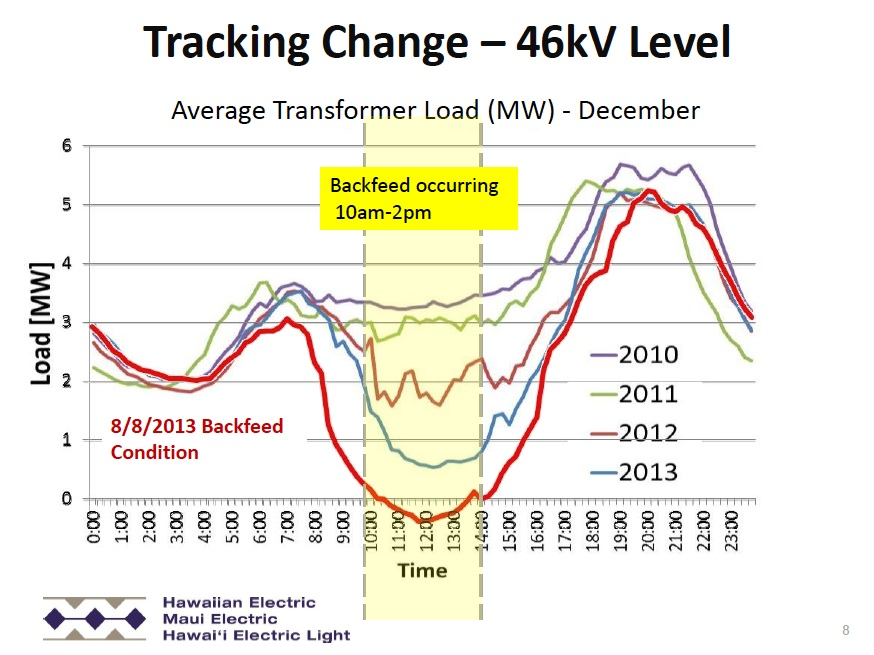
\includegraphics[scale=0.3]{images/backfeed.jpg}
\caption{The Effect of Increased Solar Adoption \cite{power:solar}}
\label{fig:solar}
\end{figure}

\subsubsection{Modelling Errors}

The model developed in Section \ref{sec:plant} is by no means a fully-accurate model of the plant.
More work will have to be done in constructing deep models of each component for the removal of the bulk of the errors.
Some other, not fully explored errors also include:
Demand data was also approximated with cubic splines to give higher resolution data for simulation.
Wind speed was approximated with cubic splines so better data at a higher resolution are required to form a more accurate model.
Wind turbine dynamics were approximated as steady state for all wind speeds and the coupling to the grid was assumed to be perfect.
A better understanding on how components couple to the electrical grid is crucial for this project to be better understood and more accurate.

\subsubsection{Grid Black-start}
\label{sec:challengespwr}

Should an event occur that knocks the grid offline, a \emph{black-start} will be required.
This is challenging as the full 230MW grid load will be drawing power at the same time, and the act of switching on the power is a step request (which acts at a high bandwidth).
Black-starts therefore take on the order of days to execute, for the UK the Restoration Time for 60\% of the grid's demand is 24 hours \cite{power:natgridblack}.
A protocol would have to be written to deal with this rare but not-impossible risk, to ensure a fast recovery from disaster.
